\documentclass[conference]{IEEEtran}
\hyphenation{op-tical net-works semi-conduc-tor}
\usepackage[bibstyle=ieee, citestyle=numeric-comp]{biblatex}
\usepackage{graphicx}
\usepackage{amsmath}
\usepackage{listings}
\usepackage{caption}
\usepackage{subcaption}
\usepackage{csquotes}
\usepackage{float}
\usepackage{color}
\usepackage{gensymb}
\usepackage{multirow}
\usepackage{array}
\usepackage{mathtools}
\usepackage[thinlines]{easytable}
\DeclarePairedDelimiter{\abs}{\lvert}{\rvert}
\usepackage[toc,page]{appendix}
\usepackage{setspace}
\usepackage{biblatex}
\addbibresource{ref.bib}
\captionsetup[figure]{labelfont={bf},labelformat={default},labelsep=period,name={Fig.}}
\addbibresource{ref.bib}
\renewcommand\IEEEkeywordsname{Keywords}

\begin{document}

\title{Suspicious Bangla Text Detection Using\\ Machine Learning}

\author{\IEEEauthorblockN{Omar Sharif}
\IEEEauthorblockA{Dept. of Computer Science \& Engineering\\
Chittagong University of Engineering and Technology\\
Chittagong-4349, Bangladesh\\
Email: omar.shaif1303@gmail.com}
\and
\IEEEauthorblockN{Mohammed Moshiul Hoque}
\IEEEauthorblockA{Dept. of Computer Science \& Engineering\\
Chittagong University of Engineering and Technology\\
Chittagong-4349, Bangladesh\\
Email: moshiulh@yahoo.com}}


\maketitle

%%%%%%% Abstract and Keyword section %%%%%%%
%%%%%%%%%%%%%%%%%%%%%%%%%%%%%%%%%%%%%%%%%%%%
\begin{abstract}
Suspicious Bangla text detection is a text classification problem of classifying Bangla text into suspicious and non suspicious category. In this paper we tried to find out the  performance of different statistical machine learning algorithm for detecting suspicious Bangla text. To the best of our knowledge, it is very first work on detecting suspicious Bangla text so we have to develop a corpus of suspicious Bangla text. This paper shows comparison of accuracy of different machine learning algorithm which will be helpful to others. The experimental result shows maximum accuracy of 92\% for Logistic Regression using 1500 training documents and 500 testing documents. The overall accuracy can be increased by increasing number of text documents in the dataset and considering semantic relation between words of a sentence.  
\end{abstract}
\vspace{0.3cm}
\begin{IEEEkeywords}
 Suspicious Bangla text, Text classification, Text classification methods, Bangla language processing, Machine learning. 
\end{IEEEkeywords}

\IEEEpeerreviewmaketitle

%%%%%%%%%% Introduction %%%%%%%%%%%%%%%%%%%%
%%%%%%%%%%%%%%%%%%%%%%%%%%%%%%%%%%%%%%%%%%%%
\section{Introduction}
Text classification is the task of assigning a text document into a set of predefined classes in an intelligent manner. Because of the rapid growth of online information, text classification has become more challenging and more important as well. Digitization has changed
the way we process and analyze information. There is an exponential increase in online availability of information. From web pages to emails, science journals, ebooks, learning content, news and social media are all full of textual data. Text classification performs an essential role in various applications that deals with organizing, classifying, searching and concisely representing a significant amount of information. Detecting suspicious text is typically a text classification problem where we have to classify a text as suspicious and not suspicious. Suspicious text detection is a kind of system where suspicious texts are identified by the keywords used in the text body. As most of our communications are text based, if we able to predict either a text is suspicious or not suspicious it will be very helpful for our law enforcement agencies to find the perpetrator and stop terrorist event. As far we know, no system is developed for detecting suspicious Bangla text. It is very important for the safety of Bangladeshi People to develop a system which can detect suspicious communications in Bangla. This motivated us to work in this area.

In this work, our original purpose is to develop a framework for detecting suspicious Bangla texts using supervised machine learning techniques. In this paper, we have applied Naïve Bayes Classifier\cite{yoo2015classification}, Support Vector Machine\cite{wei2012text, villmann2017can}, Logistic regression\cite{sharma2015active}, K-nearest neighbor algorithms (KNN)\cite{harisinghaney2014text}, Decision Trees\cite{chavan2014survey} to detect suspicious Bangla text and also find out the accuracy of this algorithms.

%%%%%%%%%% Related Work %%%%%%%%%%%%%%%%%%%%
%%%%%%%%%%%%%%%%%%%%%%%%%%%%%%%%%%%%%%%%%%%%
\section{\textbf{Related Work}}
A number of significant researches have already done in text classification in English and other language. Major works of text classification are Email classification, Research paper categorization, Detecting suspicious profiles etc.
But research on Bangla text classification is in preliminary stage still now. However some mentionable works have been done for Bangla Language Processing.
\vspace{0.2cm}

Hossain et al. describes Bengali document categorization based on word embedding and statistical learning approaches\cite{hossain2018automatic}. It categorizes document into nine predefined categories with mentionable accuracy. An Arabic text categorization system is developed using Naive Bayes in control environment dataset with good accuracy\cite{alsaleem2011automated}.
Krendzelak et al. describe a system which categorize text with machine learning and hierarchical structures by using tree based Naive Bayesian categorization process\cite{krendzelak2015text, chy2014bangla}. It performs with low accuracy due to training techniques and training feature extraction process.
\vspace{0.2cm}

S. Alami et al. describes about different techniques to detect suspicious profiles using text analysis within social media\cite{alami2015detecting}. A system for detecting suspicious email using enhanced feature selection is proposed but it has low accuracy because of not having enough dataset\cite{nizamani2013modeling}. Text Categorization of Turkish language using SVM is proposed which achieved better accuracy but due to large feature dimensions time complexity is large\cite{kaya2012sentiment}. Better result can be obtained by using clustering based approach \cite{ismail2014bangla, ahmad2016bengali} but a lot of problem exist with cluster-based solution. In our work, a system is developed and trained with different machine learning algorithms and overall accuracy of this algorithms is measured over our dataset.

%%%%%%%%% Methodology %%%%%%%%%%%%%%%%%%%%%%
%%%%%%%%%%%%%%%%%%%%%%%%%%%%%%%%%%%%%%%%%%%%
\section{\textbf{Methodology}}
The key objective of our project is to design a system that can classify suspicious and non-suspicious text. \textbf{Fig} \ref{fig:proposed_model} shows an abstract view of our suspicious text detector classifier.

\begin{figure}[h!]
\centering
  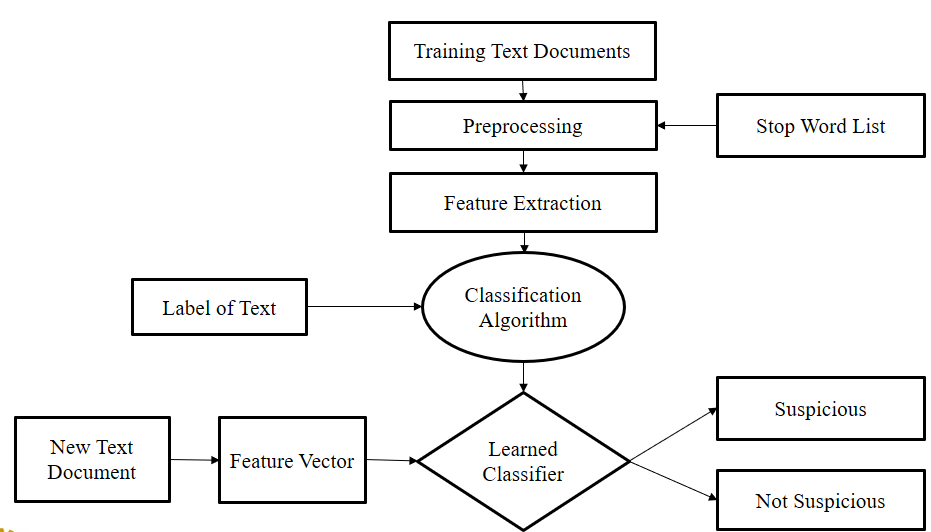
\includegraphics[scale=0.365]{Figures/proposed_model.PNG}
  \caption{ Model for Suspicious Text Detection}
  \label{fig:proposed_model}
\end{figure}

We have implemented this system by using different supervised machine learning algorithms. As a supervised classification problem, our whole system is classified into two phases one is training phase and another is testing phase.
\subsection{\textbf {Training Phase}}
In training set each document is labeled as either suspicious or non suspicious. Training phase of suspicious text detector includes five steps:
\subsubsection{\textbf{Training Set Preparation}}
Training set is divided into positive set (suspicious texts) and negative set (non suspicious texts).
\subsubsection{\textbf{Text Preprocessing}}
All texts are preprocessed by the preprocessor in order to remove inconsistencies for dataset. In our system the word which has no contribution in deciding whether a text is suspicious or not suspicious is referred as stop word. Such words are removed form the text by matching with a stop word list. 
\subsubsection{\textbf{Feature Extraction}}
A word list is created by the tokenizer by tokenizing the main body of a text. Word frequencies is used as features in this system. Bag of words model is used to represent the features. Our feature space is a two dimensional array where rows represents each text of the corpus and columns represents unique words available in the corpus. Each cell of the array represents the number of time a specific word occurs in a specific text.
\subsubsection{\textbf{Training the Suspicious Text Detector}}
It is most important part of our whole system. If we able to train our model correctly than the output will be better. Five different machine learning algorithms is used to train our model. 
\vspace{0.3cm}

\textbf{Naive Bayes}\cite{yoo2015classification} can be defined as Bayes theorem with a conditional independency assumption that all variables $A_{1},A_{2},...,A_{n}$ in a given category $C$ are conditionally independent with each other given $C$. 
According to Bayes rule for a text document $(T)$ and class $(C)$ we can write,
\begin{equation}
    P(C|T) = \frac{P(T|C)P(C)}{P(T)}
\end{equation}
The class we are looking for to assign this document is out of all classes the one that maximizes the probability of that class given the document.
\begin{equation}\label{eq:11}
 \begin{aligned}
     C_{MAP} & = argmax P(C|T) \\     & = argmax \frac{P(T|C)P(C)}{P(T)}
\end{aligned}
\end{equation}
So final equation for Naive Bayes Classifier is,
\begin{equation}
     C_{MAP} = argmax P(X_{1},X_{2},...,X_{n}|C)P(C)
\end{equation}
\vspace{0.1cm}

\textbf{SVM}\cite{wei2012text} analyze data used for classification and regression analysis. SVM can perform linear classification as well as non-linear classification using kernel trick. For linear classification cost function can be written as,
\begin{equation}
    \label{cost_function_svm}
    \frac{1}{n}\sum_{i=1}^{n}\max{(0,1-y_{i}(w.x_{i}-b))} + \lambda (\lVert \mathbf{w} \rVert)^2
\end{equation}
The parameter $\lambda $ in above equation determines the trade-off between increasing the margin-size and ensuring that the samples lie on the correct side of the margin.

For non-linear classification with SVM kernel trick is used. Some common kernel tricks used in machine learning are,
\begin{itemize}
    \item Gaussian radial basis function:
    \begin{equation}
         k(x_{i}, x_{j}) = \exp{(-\gamma(\lVert \mathbf{x_{i}-x_{j}} \rVert)^2)}
    \end{equation}
    \item Polynomial Kernel (homogeneous):
    \begin{equation}
        k(x_{i}, x_{j}) = (x_{i}\cdot x_{j})^d
    \end{equation}
     \item Polynomial Kernel (inhomogeneous):
     \begin{equation}
         k(x_{i}, x_{j}) = (x_{i}\cdot x_{j}+1)^d
     \end{equation}
\end{itemize}
\vspace{0.1cm}

A \textbf{Decision Tree}\cite{chavan2014survey} has two types of nodes one is external and another is internal. Decision classes are represented by external node of a decision tree. Internal nodes corresponds to attribute which are used for making decision by decision tree algorithm. Decision tree is simple to build and as it is a inductive algorithm it can be interpreted easily. Entropy is used to calculate the homogeneity of a sample. To build a decision tree, we need to calculate two types of entropy using as follows,
\begin{enumerate}
    \item Entropy using one attribute :
    \begin{equation}
         E(S) = \sum_{i=1}^{c}-P_i \log_2P_i
    \end{equation}
    \item Entropy using two attributes :
    \begin{equation}
        E(S) = \sum_{c\epsilon X}{}P(C)E(C) 
    \end{equation}
    
\end{enumerate}


\textbf{Logistic Regression}\cite{sharma2015active} is a binary classification model that predicts a binary outcome based on some features. The output of logistic regression depends on logistic function. The definition of logistic function or hypothesis function is,
\begin{equation}
    h_{\theta}(x) =  \frac{1}{1+\exp({-\theta^T x})}
\end{equation}
Cost function for Logistic regression is,
\begin{equation}
    J(\theta) = \frac{1}{m}\sum_{i-1}^{m}cost(h_{\theta}(x^{i}),y^{i})   
\end{equation}

\[
cost(h_{\theta}(x), y) = 
\begin{cases}
    -\log (h_{\theta}(x)) & \texttt{if } y = 1\\
     -\log (1-h_{\theta}(x)) & \texttt{if } y = 0
\end{cases}
\]
Here,\\
$m = $ Number of training examples.\\
$h_{\theta}(x^{i}) = $ Hypothesis function of $i_{th}$ training example\\
$y^i = $ Input label of $i_{th}$ training example.

\vspace{0.3cm}

\textbf{KNN}\cite{harisinghaney2014text} is a non-parametric method used for
classification and regression. K nearest neighbors is a simple algorithm that stores all available cases and classifies new cases based on a similarity measure (e.g., distance functions). Most commonly used three different distance function of K-NN are,

\begin{enumerate}
    \item Euclidean distance function :
    \begin{equation}
        \sqrt{\sum_{i=1}^{k}(x_i-y_i)^2}
    \end{equation}
    \item Manhattan distance function :
    \begin{equation}
         \sum_{i=1}^{k}\abs{(x_i-y_i)}
    \end{equation}
    \item Minkowski distance function :
    \begin{equation}
        ({\sum_{i=1}^{k}(\abs{x_i-y_i})^q)})^\frac{1}{q}
    \end{equation}
    
\end{enumerate}
All three distance measures are only valid for continuous variables.

\subsubsection{\textbf{Saving the Model}}
The result of the training phase is used in testing phase. The result is saved as a model which contains knowledge for classifying a new text document into suspicious or non suspicious category.

\subsection{\textbf{Testing Phase}}
Testing is the most important phase for any machine learning model. Classification accuracy of the text classifier is calculated in testing phase. In our system testing phase is quite similar as training phase but in this part our learned classifier model is used for predicting. Sample texts are taken to test the system. After processing, using feature extraction methods features are extracted from the texts. Our classifier model use this features to classify a text as suspicious and non suspicious.

%%%%%%%%% Experiments %%%%%%%%%%%%%%%%%%%%%%
%%%%%%%%%%%%%%%%%%%%%%%%%%%%%%%%%%%%%%%%%%%%
\section{Experiments}






















%\begin{figure}[!t]
%\centering
%\includegraphics[width=2.5in]{myfigure}
% where an .eps filename suffix will be assumed under latex, 
% and a .pdf suffix will be assumed for pdflatex; or what has been declared
% via \DeclareGraphicsExtensions.
%\caption{Simulation results for the network.}
%\label{fig_sim}
%\end{figure}

% Note that the IEEE typically puts floats only at the top, even when this
% results in a large percentage of a column being occupied by floats.


% An example of a double column floating figure using two subfigures.
% (The subfig.sty package must be loaded for this to work.)
% The subfigure \label commands are set within each subfloat command,
% and the \label for the overall figure must come after \caption.
% \hfil is used as a separator to get equal spacing.
% Watch out that the combined width of all the subfigures on a 
% line do not exceed the text width or a line break will occur.
%
%\begin{figure*}[!t]
%\centering
%\subfloat[Case I]{\includegraphics[width=2.5in]{box}%
%\label{fig_first_case}}
%\hfil
%\subfloat[Case II]{\includegraphics[width=2.5in]{box}%
%\label{fig_second_case}}
%\caption{Simulation results for the network.}
%\label{fig_sim}
%\end{figure*}
%
% Note that often IEEE papers with subfigures do not employ subfigure
% captions (using the optional argument to \subfloat[]), but instead will
% reference/describe all of them (a), (b), etc., within the main caption.
% Be aware that for subfig.sty to generate the (a), (b), etc., subfigure
% labels, the optional argument to \subfloat must be present. If a
% subcaption is not desired, just leave its contents blank,
% e.g., \subfloat[].


% An example of a floating table. Note that, for IEEE style tables, the
% \caption command should come BEFORE the table and, given that table
% captions serve much like titles, are usually capitalized except for words
% such as a, an, and, as, at, but, by, for, in, nor, of, on, or, the, to
% and up, which are usually not capitalized unless they are the first or
% last word of the caption. Table text will default to \footnotesize as
% the IEEE normally uses this smaller font for tables.
% The \label must come after \caption as always.
%
%\begin{table}[!t]
%% increase table row spacing, adjust to taste
%\renewcommand{\arraystretch}{1.3}
% if using array.sty, it might be a good idea to tweak the value of
% \extrarowheight as needed to properly center the text within the cells
%\caption{An Example of a Table}
%\label{table_example}
%\centering
%% Some packages, such as MDW tools, offer better commands for making tables
%% than the plain LaTeX2e tabular which is used here.
%\begin{tabular}{|c||c|}
%\hline
%One & Two\\
%\hline
%Three & Four\\
%\hline
%\end{tabular}
%\end{table}


% Note that the IEEE does not put floats in the very first column
% - or typically anywhere on the first page for that matter. Also,
% in-text middle ("here") positioning is typically not used, but it
% is allowed and encouraged for Computer Society conferences (but
% not Computer Society journals). Most IEEE journals/conferences use
% top floats exclusively. 
% Note that, LaTeX2e, unlike IEEE journals/conferences, places
% footnotes above bottom floats. This can be corrected via the
% \fnbelowfloat command of the stfloats package.









\renewcommand{\bibfont}{\normalfont\small}
\printbibliography

\end{document}


